\documentclass[11pt]{article}
\usepackage[margin=1in]{geometry}
\usepackage{graphicx}
\usepackage{booktabs}
\usepackage[hidelinks]{hyperref}

\title{Quantitative Facial Phenotyping Across Rare Syndromes Using Historical PRISM Measurements}
\author{Blinded for review}
\date{}

\begin{document}
\maketitle

\begin{abstract}
We analyzed 125 normalized facial measurements in 1,850 disease patients aged 3 to under 10 years and 942 distinct reference image paths. The prespecified pooled analysis included 6,125 syndrome--feature comparisons across 49 eligible syndrome groups; 811 comparisons met the global Benjamini--Hochberg threshold, including 379 with $|g| \geq 0.8$. The study is a quantitative association analysis, not an evaluation of diagnostic accuracy. [\detokenize{HUMAN_INPUT_REQUIRED}: add the clinical motivation, author-approved interpretation, and journal-length word count.]
\end{abstract}

\section{Introduction}
[\detokenize{HUMAN_INPUT_REQUIRED}: position the study against the clinical dysmorphology and quantitative phenotyping literature using verified citations. Do not infer novelty from HPO absence.]

\section{Materials and Methods}
\subsection{Study design and data sources}
Disease photographs and associated metadata were drawn from the GestaltMatcher Database (GMDB); reference photographs and labels were drawn from FairFace. The analysis compares these assembled cohorts rather than images collected under a common protocol. Disease status is therefore perfectly confounded with dataset source. Differences in acquisition, camera, lighting, compression, cropping, pose, curation, and demographic labeling cannot be estimated separately from disease--reference differences with the available data.

\subsection{Cohort construction}
The childhood analysis used the interval $3 \leq \mathrm{age} < 10$. For GMDB records, age was calculated as recorded year plus recorded month divided by 12. Year and month were required to be nonnegative integers, month was restricted to 0--11, and missing, invalid, and zero-year/zero-month records were excluded. FairFace supplied the categorical label ``3--9'' rather than exact age; all retained reference paths carried that label. Recorded ages and their cross-dataset semantics could not be independently verified.

Disease photographs first had to pass the stored frontal-quality flag. We retained one photograph per nonmissing patient identifier. For the primary selection, eligible photographs were ranked within patient by
\[
\max\left(\frac{|\mathrm{yaw}|}{15},\frac{|\mathrm{pitch}|}{15},\frac{|\mathrm{roll}|}{10}\right),
\]
with the lowest score selected and lexical image ID used to break ties. This ranking uses the historical $15^\circ/15^\circ/10^\circ$ denominators but does not reclassify the stored quality flag. The alternative photograph-selection sensitivity analysis applied the same source, quality, age, and patient eligibility rules but selected the lexically first image ID. It tests dependence on the within-patient photograph choice and is not an independent replication.

FairFace rows were restricted by the stored frontal-quality flag and deduplicated by normalized image path, removing repeated rows with the same path. Image-path uniqueness identifies distinct files, not necessarily distinct people; FairFace metadata available to this analysis did not include a participant identifier that could establish reference-participant uniqueness.

The primary syndrome analysis required at least 10 retained disease patients in a syndrome and retained the existing feature-level requirement of no more than 30\% missingness. Forty-nine syndromes met the main-analysis criterion. Demographic matched and interaction analyses used their separate computational eligibility rules: at least two disease observations in the required group or groups and at least 20 reference observations. These thresholds permit estimation but do not establish adequate power for small subgroups.

\subsection{Historical feature extraction}
The analysis uses the frozen measurements generated with the historical 125-feature FaceKit implementation at revision \texttt{e474628f3cb17a83edad59ac6e1d9e5438753032}; no newer FaceKit output is substituted. The inspected implementation converts normalized landmark coordinates to two-dimensional image pixels, centers landmarks at the midpoint of inner-canthal landmarks 133 and 362, and rotates them by the negative angle of the inner-canthal line. This is in-plane roll alignment, not yaw/pitch frontalization or three-dimensional reconstruction.

The 125 features are normalized distances, areas, angles, asymmetries, or local ratios. Normalization is formula-specific: many distances use bizygomatic width, areas often use its square, and other features use face height, midface height, mouth width, face-oval area, or a local denominator. For example, normalized philtrum length uses midface height, chin height uses face height, and cheek areas use squared bizygomatic width. Exact expressions, source locations, landmark dependencies, units, and denominators are recorded in Supplementary Table S6 and the historical formula audit. A difference in a normalized ratio can reflect its numerator, its denominator, or both and is not evidence of an absolute anatomical change.

\subsection{Statistical analysis}
For the primary pooled analysis, each of 49 eligible syndromes was compared with the reference cohort across the same 125 historical features, giving 6,125 syndrome--feature tests. The saved analysis reports Mann--Whitney tests, disease-minus-reference Hedges' $g$, and confidence intervals. One Benjamini--Hochberg (BH) correction was applied globally across all 6,125 primary tests; examples and counts in this manuscript use that global q-value rather than a within-syndrome value.

Demographic analyses were run in two harmonized layers. The broad layer combines source labels into larger groups to provide more stable cell sizes and cross-source comparability; the detailed layer preserves more of the available source-label granularity. The layers reuse observations and related mappings, so agreement between them is a sensitivity description, not independent replication. Unmapped disease records remained in the pooled analysis but were excluded from demographic comparisons. The labels are dataset annotations and should not be interpreted as precise genetic ancestry.

Analyses A, B, and C answer different questions and retain separate multiplicity families. Analysis A assesses reference-cohort variation: its omnibus BH correction spans 125 features separately within each demographic layer, while pairwise follow-up correction is performed within pair. Analysis B compares disease and reference observations within a demographic group and uses a global BH family separately for the broad and detailed layers. Analysis C tests whether the disease--reference difference varies between two groups and likewise uses a separate global BH family within each layer. Counts from these families are not additive.

For Analysis C, the formal interaction test is the disease-by-group coefficient from the interaction model, reported with an HC3 robust standard error, confidence interval, and the Analysis C global q-value. Group-specific Hedges' $g$ values and their difference ($\Delta g$) are descriptive and are not substituted for the interaction coefficient. A sign reversal in descriptive effects is not by itself evidence of interaction.

Three predefined recorded-covariate sensitivity models were also fit for highlighted syndrome--feature pairs using complete-case ordinary least squares with HC3 robust standard errors. These models included sex label, broad demographic group, yaw, pitch, and roll and applied BH correction across the three predefined models. Exact-age adjustment was not possible because FairFace provides an age category rather than exact age. These exploratory models assess sensitivity to recorded covariates only; they neither replace the primary Mann--Whitney analysis nor resolve unmeasured acquisition differences or the perfect confounding of disease status with dataset source.

\section{Results}
\subsection{Cohort and primary analysis}
Of 10,942 disease-image records, 9,411 carried a passing stored frontal-quality flag and 2,101 of those met the recorded childhood age rule. Removing 251 additional photographs from patients with more than one eligible image left 1,850 disease patients with one selected photograph each. Deduplication of the reference cohort left 942 distinct FairFace image paths. Forty-nine syndrome groups met the minimum disease-group size, producing 6,125 primary tests across 125 features.

The primary analysis contained 811 globally significant comparisons (13.2\% of 6,125), of which 379 met $|g| \geq 0.8$. Among globally significant rows, 490 effects were positive and 321 were negative under the stored disease-minus-reference sign convention. These are counts of correlated normalized measurements, not counts of independent biological discoveries. Figure~\ref{fig:cross-syndrome} summarizes selected cross-syndrome effects without assigning a clinical or literature classification.

\begin{figure}[htbp]
  \centering
  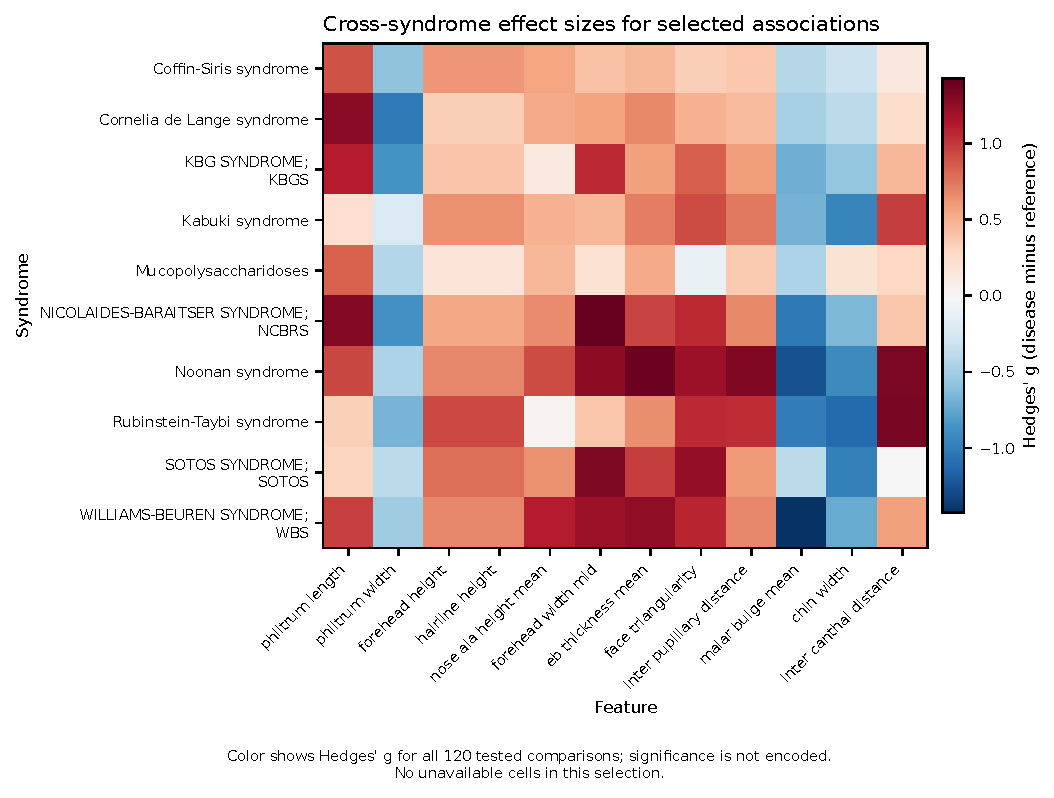
\includegraphics[width=\linewidth]{figures/fig1_cross_syndrome_heatmap.pdf}
  \caption{Cross-syndrome Hedges' $g$ values for selected associations. Source values are supplied with the publication package.}
  \label{fig:cross-syndrome}
\end{figure}

\subsection{Demographic analyses}
Reference-group omnibus tests were significant for 72 of 125 features in the broad layer and 89 of 125 in the detailed layer (Figure~\ref{fig:reference}). Analysis B contained 36,000 broad-layer tests with 375 global-BH-significant results and 33,875 detailed-layer tests with 452 significant results. Analysis C contained 11,500 broad-layer tests with 479 global-BH-significant interaction coefficients and 15,000 detailed-layer tests with 633 significant interaction coefficients. These totals belong to separate correction families, use overlapping observations, and should not be summed or treated as replication across layers.

\begin{figure}[htbp]
  \centering
  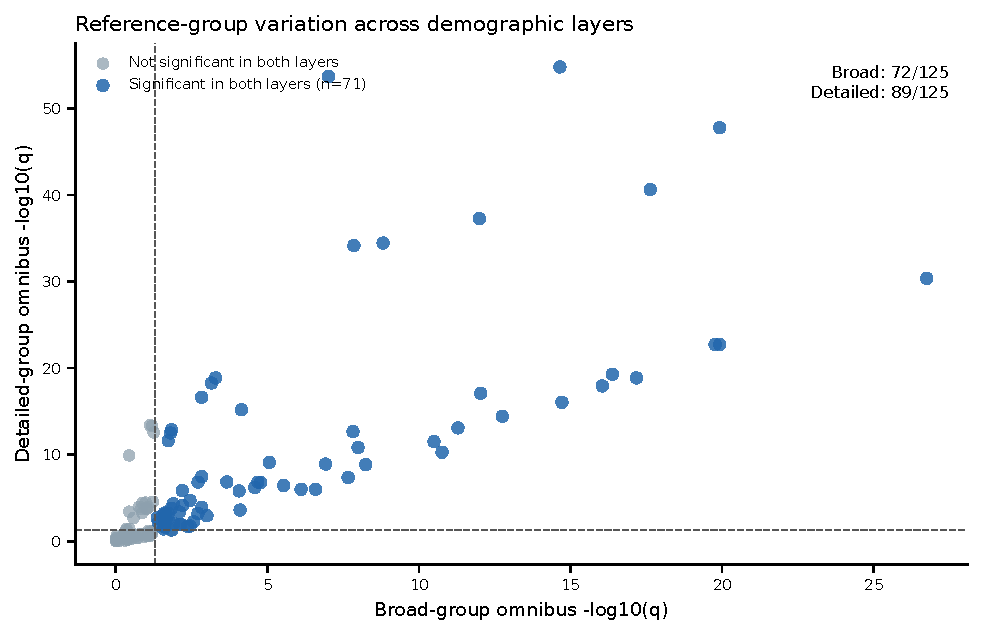
\includegraphics[width=0.9\linewidth]{figures/fig2_reference_variation.pdf}
  \caption{Reference-group omnibus q-values in broad and detailed demographic layers. Dashed lines mark $q=0.05$.}
  \label{fig:reference}
\end{figure}

\subsection{Photograph-selection sensitivity}
The alternative selection changed the retained photograph for 94 of 1,850 disease patients (5.1\%). It yielded 834 comparisons meeting the global BH threshold, compared with 811 under the primary selection. The selections shared 770 significant comparisons; 41 were primary-only and 64 were alternative-only. Thus, 94.9\% of primary significant findings were retained and the significant-set Jaccard overlap was 88.0\% (Figure~\ref{fig:selection}). This analysis changes only within-patient photograph selection and does not provide an external cohort or independent replication.

\begin{figure}[htbp]
  \centering
  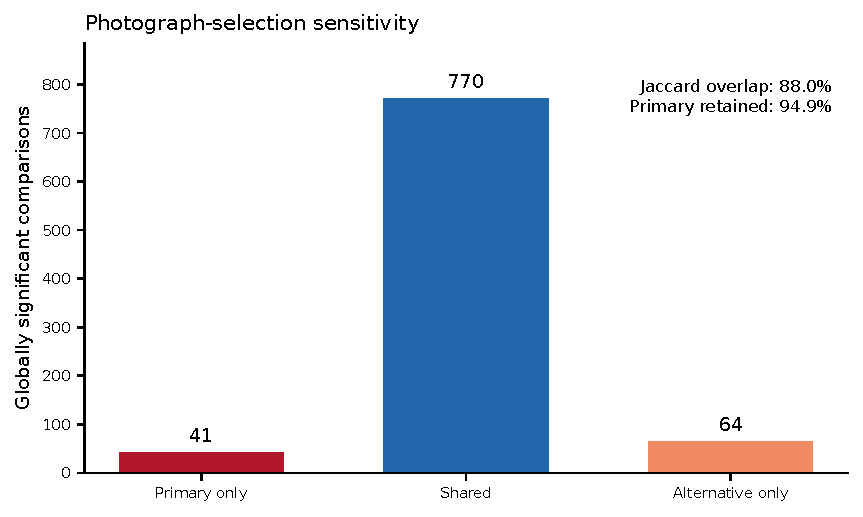
\includegraphics[width=0.85\linewidth]{figures/fig3_selection_overlap.pdf}
  \caption{Overlap of globally significant pooled comparisons under primary and alternative photograph selection. This is a sensitivity analysis, not independent replication.}
  \label{fig:selection}
\end{figure}

\section{Discussion}
[\detokenize{HUMAN_INPUT_REQUIRED}: add a literature-verified and clinician-reviewed interpretation. Do not classify candidate associations, claim novelty, or convert correlated significant measurements into independent discoveries until that review is recorded.]

\section{Limitations}
Reference image-path uniqueness does not establish participant uniqueness. Recorded ages are not independently verified. Small demographic subgroups can yield unstable estimates. The disease and reference cohorts come from different datasets, leaving disease status confounded with acquisition and curation source. Normalized ratios do not isolate absolute changes in their numerators.

\section{Conclusion}
[\detokenize{HUMAN_INPUT_REQUIRED}: provide an author-approved conclusion limited to quantitative association and reproducibility.]

\section{Data and Code Availability}
The publication package records source hashes and regeneration scripts. The repository is currently private, and this manuscript makes no claim that source-level, patient/image-level, per-image derived, aggregate, code, or historical Git content is approved for public redistribution. [\detokenize{HUMAN_INPUT_REQUIRED}: insert mentor-, institution-, and data-provider-approved data/code availability language and the authorized public-release boundary.]

\section{Ethics Statement}
[\detokenize{HUMAN_INPUT_REQUIRED}: insert the institution-approved ethics, consent, exemption, and oversight language.]

\section{Funding}
[\detokenize{HUMAN_INPUT_REQUIRED}: insert funding sources and grant identifiers, or an approved no-funding statement.]

\section{Conflicts of Interest}
[\detokenize{HUMAN_INPUT_REQUIRED}: insert the author- and journal-approved conflicts-of-interest statement.]

\section{Author Contributions}
[\detokenize{HUMAN_INPUT_REQUIRED}: insert contribution roles after all authors approve them.]

\section{References}
[\detokenize{HUMAN_INPUT_REQUIRED}: add only verified references to \texttt{references.bib} and cite them in the text.]

\section{Supplementary Information}
Supplementary Tables S1--S6 provide the pooled associations, reference variation, matched comparisons, formal interactions, photograph-selection sensitivity, and feature definitions. The candidate evidence table and feature-redundancy report are also supplied in the publication package.

[\detokenize{HUMAN_INPUT_REQUIRED}: review and approve the exact historical feature-definition supplement before submission.]

\end{document}
